\documentclass[a4paper, 12pt]{article}

% 导入必要的包
\usepackage{graphicx}    % 图片支持
\usepackage{ctex}        % 中文支持
\usepackage{amsmath}     % 数学公式
\usepackage{amssymb}     % 数学符号
\usepackage{mathtools}   % 增强的数学工具
\usepackage{booktabs}    % 表格
\usepackage{hyperref}    % 超链接
\usepackage{natbib}      % 参考文献
\usepackage{geometry}    % 页面设置
\usepackage{fancyhdr}    % 页眉页脚
\usepackage{subfig}      % 子图支持

% 数学符号定义
\DeclareMathOperator*{\E}{\mathbb{E}}    % 期望算子
\newcommand{\KL}{\text{KL}}              % KL散度

% 页面设置
\geometry{left=2.5cm,right=2.5cm,top=2.5cm,bottom=2.5cm}
\pagestyle{fancy}
\fancyhf{}
\rhead{基于GRPO的坐标序列预测实验报告}
\lfoot{\thepage}

% 文档信息
\title{
    
\includegraphics[width=1\textwidth]{Images/icon.png}\\[1cm]
    \Huge 基于GRPO的坐标序列预测\\[0.5cm]
    \Large 自然语言处理课程项目\\[0.5cm]
    \Large 浙江大学计算机科学与技术学院
}
\author{
    \vspace{1cm}
    \begin{tabular}{lr}
        王\hspace{2em}阳 & (贡献度:35\%)\\[0.3cm]
        周齐圣 & (贡献度:25\%)\\[0.3cm]
        刘\hspace{2em}涵 & (贡献度:20\%)\\[0.3cm]
        郑思华 & (贡献度:20\%)
    \end{tabular}
}
\date{2025年6月15日}

\begin{document}

% 封面
\maketitle
\thispagestyle{empty}

% 目录
\newpage
\tableofcontents
\newpage

% 第一章:任务介绍
\section{任务介绍}
\subsection{项目背景}
近年来,强化学习在自然语言处理领域的应用取得了显著进展\cite{rl_nlp2021}。与传统的监督学习不同,强化学习不需要直接给定标签进行学习,而是通过构造奖励函数来指导模型的学习方向。这种方法在特定任务中展现出了独特的优势。

本项目探索了将GRPO(Generative Reward Processing and Optimization)算法\cite{grpo2024}应用于坐标序列预测任务的可能性。GRPO作为一种新型的强化学习算法,其特点是通过构造奖励函数来评估模型生成结果的合理性,从而优化模型的推理过程。在本项目中,我们将这一算法应用于预测符合特定运动规律的坐标序列,这不仅能验证算法的有效性,也能探索其在数值预测任务中的应用潜力。

\subsection{项目目标}
本项目的具体目标包括以下几个方面:

\subsubsection{数据构建}
构造符合一维匀速直线运动规律的坐标数据:
\begin{itemize}
    \item \textbf{运动类型}:一维匀速直线运动,形如 $\{(x_1), (x_1+v\cdot\Delta t), \ldots, (x_1+v\cdot n\Delta t)\}$
    \item \textbf{数据特点}:
        \begin{itemize}
            \item 初始位置 $x_1$ 和速度 $v$ 均为浮点数
            \item 时间间隔 $\Delta t$ 固定为1个单位时间
            \item 序列长度为10个点(给定前5个点,预测后5个点)
        \end{itemize}
    \item \textbf{数据要求}:构造具有不同速度范围的训练和测试数据,以验证模型的泛化能力
\end{itemize}

\subsubsection{算法实现}
基于以下技术栈实现坐标序列预测系统:
\begin{itemize}
    \item \textbf{强化学习算法}:采用GRPO\cite{grpo2024},基于HuggingFace的open-r1\cite{openr1}实现
    \item \textbf{基础模型}:使用Qwen2.5-1.5B-Instruct\cite{qwen2024}作为backbone模型
    \item \textbf{预测任务}:给定5个连续坐标点,预测后续5个坐标点的位置
\end{itemize}

\subsubsection{实验验证}
设计完整的实验验证方案:
\begin{itemize}
    \item \textbf{数据划分}:
        \begin{itemize}
            \item 训练集:50组序列,速度范围在[0.5, 2.0]之间
            \item 测试集:分为两类
                \begin{itemize}
                    \item In-distribution:20组序列,速度范围与训练集相同
                    \item Out-of-distribution:20组序列,速度范围在[2.0, 3.0]之间
                \end{itemize}
        \end{itemize}
    \item \textbf{预测要求}:模型需要通过分析给定的5个点,推理出运动规律,并准确预测后续5个点的位置
\end{itemize}

\subsubsection{评估指标}
主要从以下几个方面评估模型性能:
\begin{itemize}
    \item \textbf{预测准确性}:评估模型预测的5个坐标点与真实值的误差
    \item \textbf{泛化能力}:比较模型在不同速度范围数据上的表现差异
    \item \textbf{推理过程}:分析模型的chain-of-thought能力,评估其对运动规律的理解
\end{itemize}

% 第二章:算法介绍
\section{算法介绍}
\subsection{强化学习基础}
强化学习是机器学习的一个重要分支,其核心思想是通过智能体(Agent)与环境(Environment)的交互来学习最优策略。在传统的监督学习中,模型通过已标注的数据直接学习输入到输出的映射。而在强化学习中,模型通过与环境的交互获得反馈(奖励),从而逐步优化其行为策略。

\subsubsection{基本框架}
强化学习的基本流程如图\ref{fig:rl_framework}所示,主要包含以下关键要素:

\begin{figure}[htbp]
    \centering
    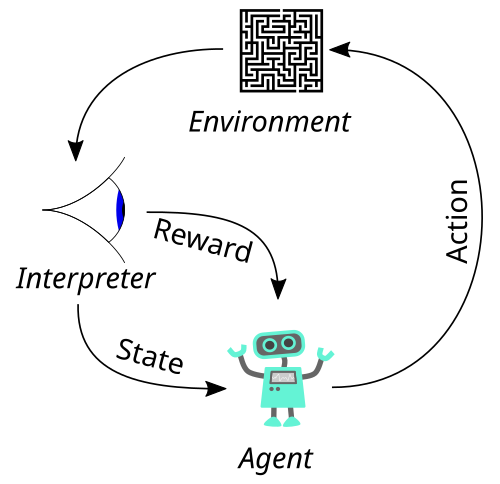
\includegraphics[width=0.5\textwidth]{Images/RL.png}
    \caption{强化学习基本框架}
    \label{fig:rl_framework}
\end{figure}

\begin{itemize}
    \item \textbf{状态空间}(State Space)$\mathcal{S}$:描述环境在某一时刻的状态,在本项目中表示为已知的坐标序列
    \item \textbf{动作空间}(Action Space)$\mathcal{A}$:智能体可以采取的所有可能行动,在本项目中对应模型生成的预测序列
    \item \textbf{转移函数}(Transition Function)$P(s_{t+1}|s_t,a_t)$:描述在当前状态下采取某个动作后环境状态的变化
    \item \textbf{奖励函数}(Reward Function)$R(s_t,a_t)$:评估智能体在某个状态下采取特定动作的好坏,本项目中包含预测准确性和推理过程的评估
    \item \textbf{策略}(Policy)$\pi(a|s)$:决定智能体在特定状态下应该采取什么动作,在本项目中即为模型的生成策略
\end{itemize}

\subsubsection{学习过程}
强化学习的核心目标是最大化累积奖励,其学习过程主要包含以下步骤:

\begin{enumerate}
    \item \textbf{状态观察}:智能体观察当前环境状态 $s_t$
    \item \textbf{动作选择}:根据策略 $\pi(a|s)$ 选择动作 $a_t$
    \item \textbf{环境交互}:执行动作并获得奖励 $r_t$ 和新状态 $s_{t+1}$
    \item \textbf{策略更新}:基于获得的奖励更新策略,优化目标为:
        \begin{equation}
            J(\theta) = \E_{\tau \sim \pi_\theta}[\sum_{t=0}^{T} \gamma^t r_t]
        \end{equation}
        其中 $\gamma$ 为折扣因子,$\tau$ 表示交互轨迹
\end{enumerate}

\subsubsection{在NLP中的应用}
在自然语言处理领域,强化学习的应用具有其特殊性:
\begin{itemize}
    \item \textbf{状态表示}:通常是文本序列或模型的隐状态,需要考虑文本的语义和结构信息
    \item \textbf{动作空间}:往往是离散的词表或token空间,这使得动作空间非常大且稀疏
    \item \textbf{奖励设计}:需要考虑多个方面:
        \begin{itemize}
            \item \textbf{任务相关}:如预测准确性、生成质量等
            \item \textbf{语言特性}:如语法正确性、语义连贯性等
            \item \textbf{推理能力}:如逻辑性、可解释性等
        \end{itemize}
    \item \textbf{训练挑战}:
        \begin{itemize}
            \item 奖励稀疏性:有效的奖励信号可能很少
            \item 探索效率:在大规模动作空间中进行有效探索
            \item 训练稳定性:需要特殊的技术来保持训练的稳定性
        \end{itemize}
\end{itemize}

\subsection{GRPO算法}
\subsubsection{算法概述}
GRPO(Generative Reward Processing and Optimization)\cite{grpo2024}是一种专门针对大语言模型的强化学习算法。如图\ref{fig:grpo_framework}所示,与传统的PPO(Proximal Policy Optimization)算法相比,GRPO通过创新的设计显著降低了训练资源的需求,同时保持了较好的训练效果。

\begin{figure}[htbp]
    \centering
    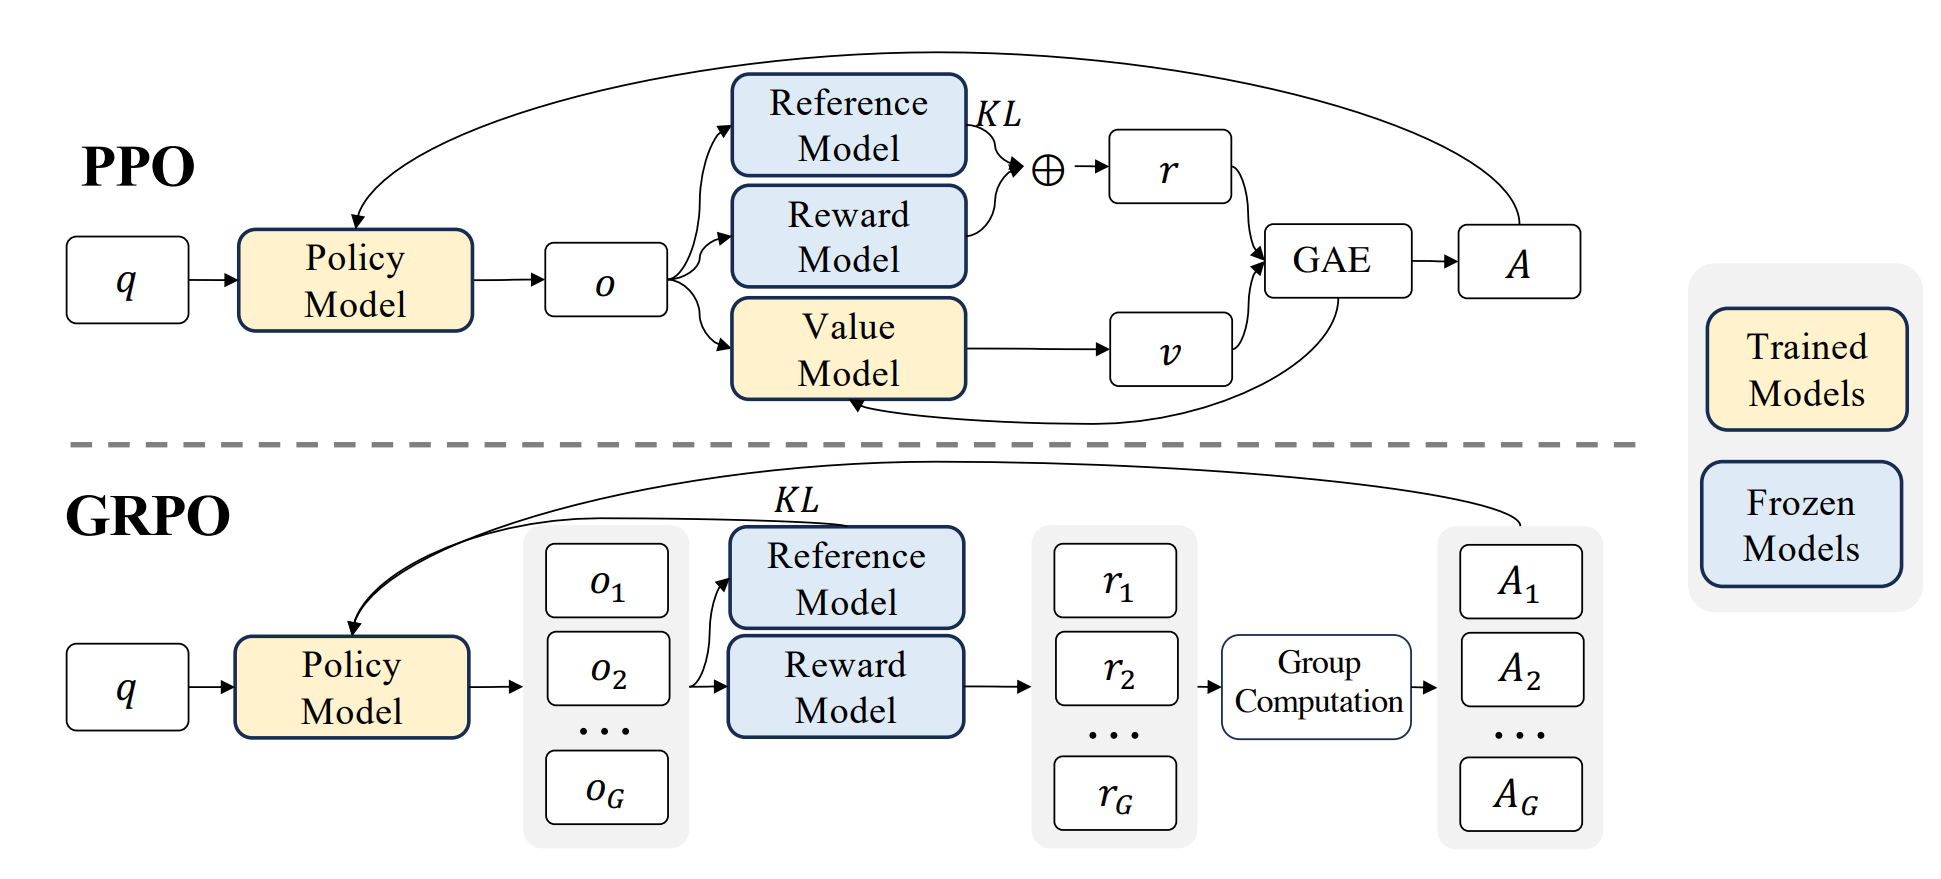
\includegraphics[width=0.9\textwidth]{Images/GRPO.png}
    \caption{GRPO与PPO算法对比图。GRPO省略了价值模型,而是通过组内评分估计基线,显著减少了训练资源需求。}
    \label{fig:grpo_framework}
\end{figure}

GRPO算法的主要创新点包括:
\begin{itemize}
    \item \textbf{无价值网络设计}:传统PPO算法需要训练一个额外的价值网络来估计状态价值,而GRPO直接利用组内样本的奖励分数来估计基线,大大减少了计算开销
    \item \textbf{生成式奖励处理}:利用语言模型自身的能力来理解和处理奖励信号,使奖励更加灵活和可解释
    \item \textbf{多样性保持}:通过KL散度约束和组采样机制,在优化过程中保持输出的多样性
    \item \textbf{稳定性提升}:采用特殊的优化策略来提高训练的稳定性
\end{itemize}

\subsubsection{算法流程}
GRPO的训练流程主要包含以下步骤:

\begin{enumerate}
    \item \textbf{组采样}:
        \begin{itemize}
            \item 对于每个输入状态 $s$,从当前策略 $\pi_\theta$ 采样 $K$ 个动作(生成结果)
            \item 形成动作组 $\{a_1, a_2, ..., a_K\}$,每个动作代表一个可能的预测序列
        \end{itemize}
    
    \item \textbf{奖励计算}:
        \begin{itemize}
            \item 对组内每个动作计算奖励 $R(s,a_k)$
            \item 基线估计:$b(s) = \frac{1}{K}\sum_{k=1}^K R(s,a_k)$
            \item 计算优势:$A(s,a_k) = R(s,a_k) - b(s)$
        \end{itemize}
    
    \item \textbf{策略更新}:
        \begin{equation}
            \mathcal{L}_{\text{GRPO}} = \E_{s \sim \mathcal{D}, a \sim \pi_\theta}[R(s,a)] - \alpha \KL(\pi_\theta \| \pi_{\text{ref}})
        \end{equation}
        其中:
        \begin{itemize}
            \item $\pi_\theta$:当前策略(待优化的模型)
            \item $\pi_{\text{ref}}$:参考策略(原始预训练模型)
            \item $\alpha$:KL散度权重,用于控制策略更新的幅度
        \end{itemize}
\end{enumerate}

% 第三章:实验设计
\section{实验设计}
\subsection{数据准备}
本实验的数据集由自行构造的坐标序列组成,主要包含以下几个方面:

\subsubsection{数据生成}
我们设计了一个数据生成器(\texttt{MotionDataGenerator}),用于生成符合特定运动规律的坐标序列。生成器的主要特点如下:

\begin{itemize}
    \item \textbf{运动类型}:一维匀速直线运动,通过以下公式生成:
        \begin{equation}
            x_t = x_0 + v \cdot t, \quad t \in \{0,1,\ldots,n-1\}
        \end{equation}
        其中 $x_0$ 为初始位置,$v$ 为速度,$n$ 为序列长度
    
    \item \textbf{参数配置}:根据配置文件设置不同数据集的参数范围
        \begin{itemize}
            \item 训练集(50组序列):
                \begin{itemize}
                    \item 初始速度 $v_0 \in [0.5, 2.0]$
                    \item 加速度范围 $a \in [0.1, 0.5]$
                \end{itemize}
            \item In-distribution测试集(20组序列):
                \begin{itemize}
                    \item 参数范围与训练集相同
                \end{itemize}
            \item Out-of-distribution测试集(20组序列):
                \begin{itemize}
                    \item 初始速度 $v_0 \in [2.0, 3.0]$
                    \item 加速度范围 $a \in [0.5, 1.0]$
                \end{itemize}
        \end{itemize}
    
    \item \textbf{序列生成}:每个序列包含10个点
        \begin{itemize}
            \item 输入序列:前5个点作为模型输入
            \item 目标序列:后5个点作为预测目标
        \end{itemize}
\end{itemize}

\subsubsection{数据格式}
为了激活模型的chain-of-thought能力,我们为每个数据样本设计了特定的格式:

\begin{itemize}
    \item \textbf{输入提示}:包含以下组成部分
        \begin{itemize}
            \item 任务说明和格式要求
            \item 示例分析过程,包含:
                \begin{itemize}
                    \item [Analysis]标签:详细的推理步骤
                    \item [ANSWER]标签:预测结果
                    \item [End]标签:结果终止标记
                \end{itemize}
            \item 待分析的坐标序列(格式化为带一位小数的坐标点)
        \end{itemize}
    
    \item \textbf{目标输出}:后续5个坐标点,格式化为带一位小数的形式
        \begin{itemize}
            \item 示例:(9.5), (11.0), (12.5), (14.0), (15.5)
        \end{itemize}
\end{itemize}

\subsubsection{数据处理}
数据生成和处理流程的实现采用了模块化设计:

\begin{itemize}
    \item \texttt{generator.py}:核心数据生成器
        \begin{itemize}
            \item \texttt{generate\_sequence}:生成单个运动序列
            \item \texttt{format\_coordinates}:格式化坐标为输入输出对
            \item \texttt{generate\_dataset}:批量生成数据集
        \end{itemize}
    \item \texttt{config.yaml}:集中管理数据生成参数
        \begin{itemize}
            \item 各数据集的样本数量配置
            \item 运动参数范围设置
            \item 训练相关超参数配置
        \end{itemize}
\end{itemize}

\subsection{奖励函数设计}
在本项目中,我们设计了两个独立的奖励函数来评估模型的输出质量:准确性奖励(Accuracy Reward)和格式奖励(Format Reward)。

\subsubsection{准确性奖励}
该奖励函数专注于评估预测坐标的准确性:
\begin{itemize}
    \item \textbf{计算方法}:使用均方误差(MSE)评估预测坐标与目标坐标的差异
        \begin{equation}
            \text{accuracy} = \exp(-\text{MSE}(y_{\text{pred}}, y_{\text{target}}))
        \end{equation}
    \item \textbf{评分规则}:
        \begin{itemize}
            \item 正好预测5个坐标:完整准确度分数
            \item 少于5个坐标:分数按比例降低,$\text{score} = \text{accuracy} \times 0.8 \times \frac{n_{\text{pred}}}{5}$
            \item 多于5个坐标:分数略微降低,$\text{score} = \text{accuracy} \times 0.9$
        \end{itemize}
    \item \textbf{格式要求}:必须包含正确的标签([Analysis], [ANSWER], [End])且顺序正确
\end{itemize}

\subsubsection{格式奖励}
该奖励函数评估输出的格式规范性,总分为1.0,包含三个方面:
\begin{itemize}
    \item \textbf{基本结构}(0.4分):
        \begin{itemize}
            \item 必需标签的存在性:[Analysis], [ANSWER], [End]
            \item 标签顺序的正确性
        \end{itemize}
    \item \textbf{分析步骤格式}(0.3分):
        \begin{itemize}
            \item S1-S3步骤的完整性(0.1分)
            \item $\Delta x$ 计算格式的规范性(0.1分)
            \item 速度计算格式的规范性(0.1分)
        \end{itemize}
    \item \textbf{答案格式}(0.3分):
        \begin{itemize}
            \item 预测坐标数量为5个(0.2分)
            \item 坐标格式和分隔符的规范性(0.1分)
        \end{itemize}
\end{itemize}

\subsubsection{综合奖励}
最终的奖励值是两个奖励函数的加权和:
\begin{equation}
    R_{\text{total}} = w_1 \cdot R_{\text{accuracy}} + w_2 \cdot R_{\text{format}}
\end{equation}
其中权重比例为 $w_1 : w_2 = 5 : 1$,以确保模型优先关注预测的准确性,同时保持输出格式的规范性。

\subsection{实验框架}
本实验基于HuggingFace的open-r1框架实现,采用模块化设计,整体框架如下:

\subsubsection{项目结构}
项目采用标准的Python包结构:
\begin{itemize}
    \item \texttt{src/}:核心源代码目录
        \begin{itemize}
            \item \texttt{data/}:数据处理模块
                \begin{itemize}
                    \item \texttt{generator.py}:坐标序列生成器,实现数据生成和格式化
                    \item \texttt{dataset.py}:数据集加载和预处理接口
                \end{itemize}
            \item \texttt{models/}:模型实现
                \begin{itemize}
                    \item \texttt{qwen\_model.py}:Qwen2.5-1.5B-Instruct模型的封装和配置
                \end{itemize}
            \item \texttt{utils/}:工具函数
                \begin{itemize}
                    \item \texttt{reward.py}:奖励函数计算
                    \item \texttt{metrics.py}:评估指标实现
                \end{itemize}
        \end{itemize}
    \item \texttt{scripts/}:运行脚本
        \begin{itemize}
            \item \texttt{generate\_data.py}:数据生成脚本
        \end{itemize}
    \item \texttt{config/}:配置文件
        \begin{itemize}
            \item \texttt{config.yaml}:实验参数配置,包括:
                \begin{itemize}
                    \item 数据生成参数
                    \item 模型训练参数
                    \item 实验记录配置
                \end{itemize}
        \end{itemize}
\end{itemize}

\subsubsection{实验配置}
根据\texttt{config.yaml}的具体配置:

\begin{itemize}
    \item \textbf{模型配置}:
        \begin{itemize}
            \item 模型路径:\texttt{/root/NLP2025/Qwen}
            \item 最大序列长度:800 tokens
            \item 生成参数:
                \begin{itemize}
                    \item 温度系数:0.7
                    \item top-p:0.9
                    \item 每个输入生成4个候选结果
                \end{itemize}
        \end{itemize}
    
    \item \textbf{训练配置}:
        \begin{itemize}
            \item 学习率:$1 \times 10^{-6}$
            \item 训练轮数:10轮
            \item 批处理大小:8
            \item 梯度累积步数:4
            \item 启用FP16混合精度训练
        \end{itemize}
    
    \item \textbf{GRPO特定参数}:
        \begin{itemize}
            \item $\beta$ 系数:0.04
            \item $\epsilon$ 阈值:0.2
            \item 迭代次数:1
            \item 损失类型:BNPO(Batch Normalized Policy Optimization)
            \item 奖励权重:[5, 1](准确性vs多样性)
        \end{itemize}
    
    \item \textbf{实验记录}:
        \begin{itemize}
            \item 日志目录:\texttt{./logs}
            \item 指标更新间隔:每10步
            \item 模型保存间隔:每200步
            \item 保存策略:仅保留最新的2个检查点
            \item 使用safetensors格式保存模型
        \end{itemize}
\end{itemize}

\subsubsection{提示工程}
基于\texttt{generator.py}中的实现,我们设计了结构化的提示模板:

\begin{verbatim}
Please follow the exact format of the example below to analyze the coordinates and make predictions.
Your answer must contain [Analysis], [ANSWER], and [End] tags, with the final 5 predicted coordinates between [ANSWER] and [End] tags.

Example:
Input: (2.0), (3.5), (5.0), (6.5), (8.0)

[Analysis]
S1: Checking motion pattern
   Δx1 = 3.5 - 2.0 = 1.5
   Δx2 = 5.0 - 3.5 = 1.5
   Δx3 = 6.5 - 5.0 = 1.5
   Δx4 = 8.0 - 6.5 = 1.5
   All intervals are approximately equal ≈ 1.5

S2: Speed = Average(Δx/Δt) = 1.5 units/step

S3: Prediction using average speed
   Starting from x₀ = 8.0
   x = x₀ + v·t = 8.0 + 1.5t

[ANSWER]
(9.5), (11.0), (12.5), (14.0), (15.5)
[End]

Now analyze: {input_coordinates}
\end{verbatim}

该模板的设计考虑了以下几个方面:
\begin{itemize}
    \item \textbf{结构化分析}:要求模型按步骤进行分析,便于评估推理过程
    \item \textbf{标准化输出}:使用特定标签标记不同部分,便于结果提取
    \item \textbf{示例引导}:通过具体示例展示期望的分析方式和格式
    \item \textbf{精度控制}:统一使用一位小数的格式化输出
\end{itemize}

% 第四章:实验结果
\section{实验结果}
\subsection{训练过程分析}
在120轮训练过程中,我们主要关注两个关键指标的变化:准确性奖励(Accuracy Reward)和格式奖励(Format Reward)。这两个指标分别反映了模型在预测精度和输出规范性方面的表现。

\begin{figure}[htbp]
    \centering
    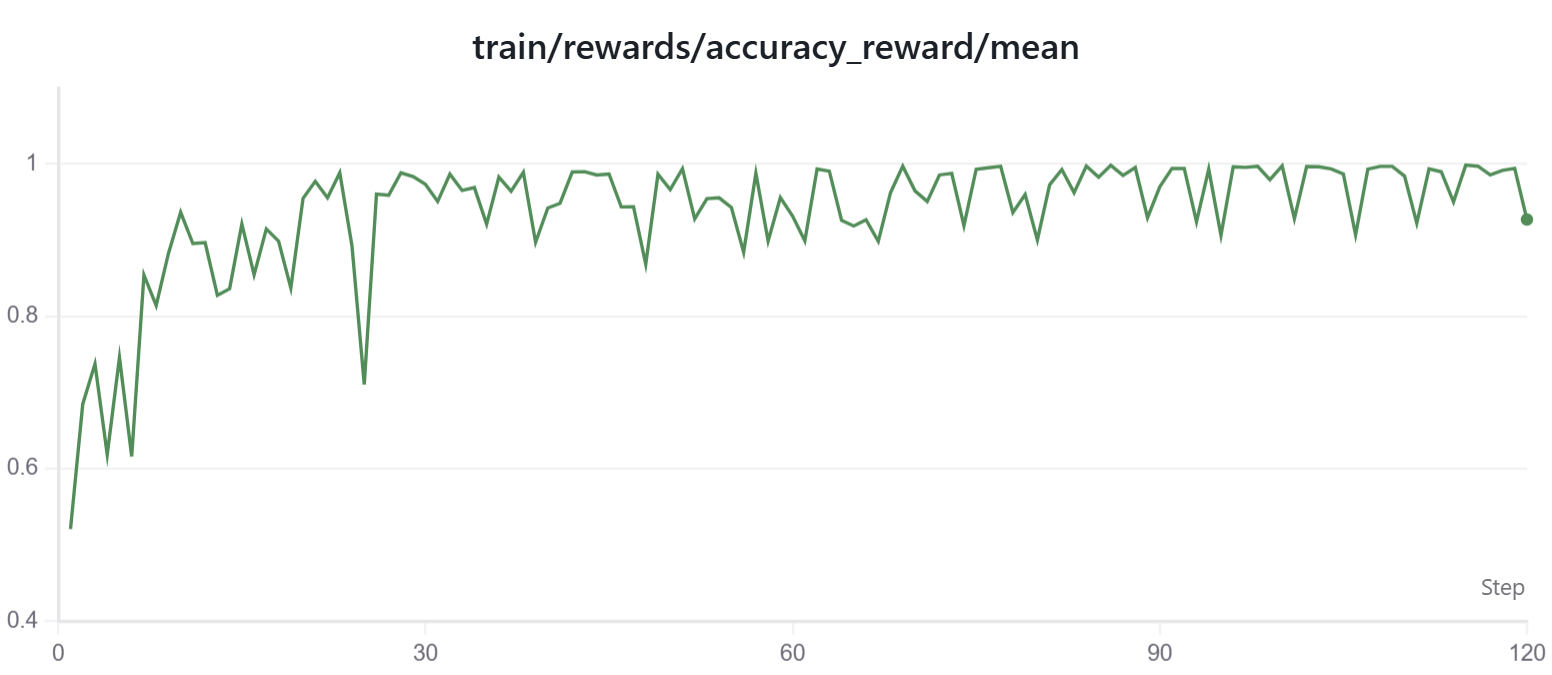
\includegraphics[width=0.8\textwidth]{Images/accuracy_reward.png}
    \caption{训练过程中准确性奖励的变化趋势}
    \label{fig:accuracy_reward}
\end{figure}

如图\ref{fig:accuracy_reward}所示,准确性奖励在训练过程中呈现以下特点:
\begin{itemize}
    \item \textbf{初始阶段}(0-30轮):奖励值波动较大,表明模型在适应任务
    \item \textbf{快速提升阶段}(30-60轮):奖励值显著提升,模型开始掌握预测规律
    \item \textbf{稳定阶段}(60-120轮):奖励值趋于稳定,波动减小,说明模型达到了较好的预测能力
\end{itemize}

\begin{figure}[htbp]
    \centering
    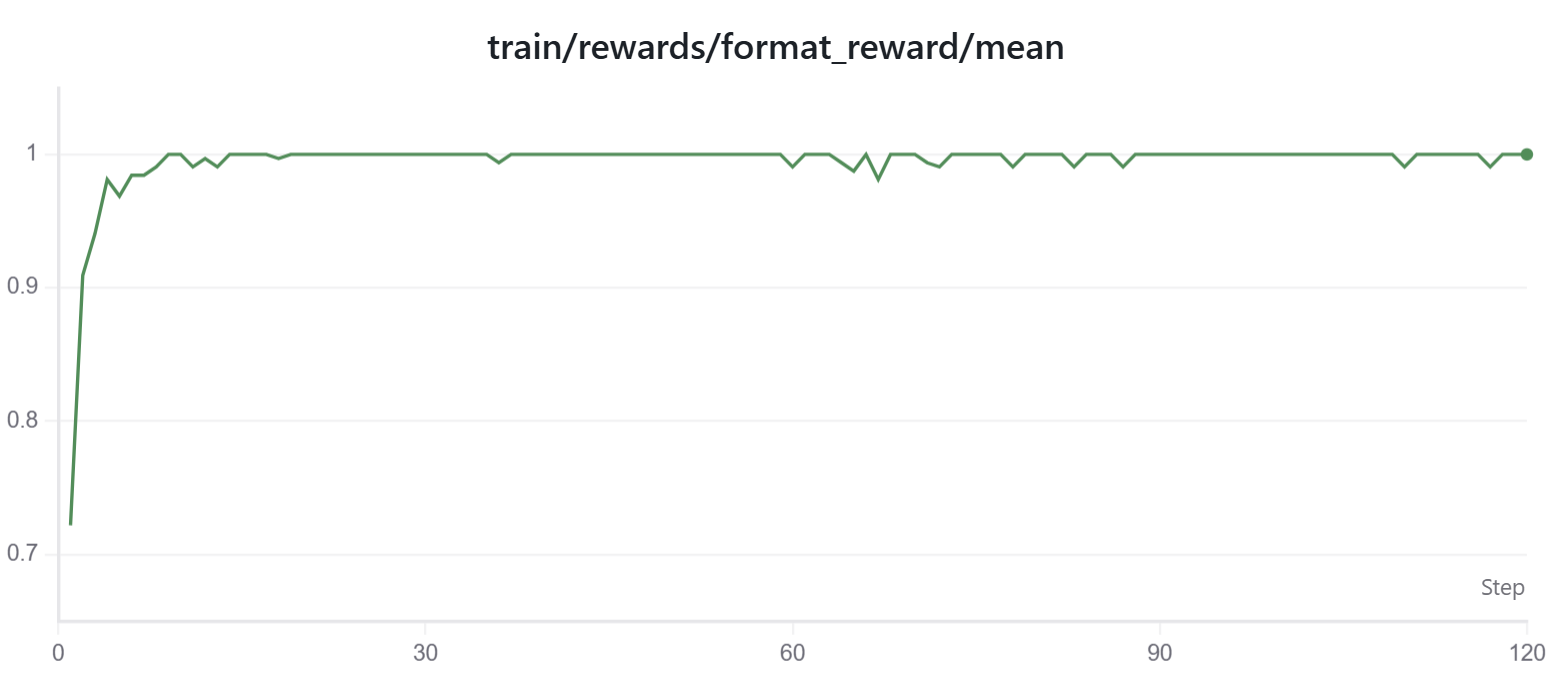
\includegraphics[width=0.8\textwidth]{Images/format_reward.png}
    \caption{训练过程中格式奖励的变化趋势}
    \label{fig:format_reward}
\end{figure}

图\ref{fig:format_reward}展示了格式奖励的变化趋势:
\begin{itemize}
    \item \textbf{快速收敛}:格式奖励在训练初期就达到较高水平,说明模型很快掌握了输出格式要求
    \item \textbf{高度稳定}:整个训练过程中波动很小,表明模型能够持续保持良好的输出规范性
    \item \textbf{轻微优化}:在后期仍有小幅提升,显示模型在细节方面的持续改进
\end{itemize}

综合两个指标的变化可以看出:
\begin{itemize}
    \item 模型在格式学习方面表现出色,这得益于提示模板的良好设计
    \item 预测准确性的提升需要更多训练轮次,这符合任务的难度特征
    \item 两个指标最终都达到了稳定状态,说明训练轮次的设置是合理的
\end{itemize}

\subsection{测试结果分析}
为了详细评估模型的预测性能,我们分别对in-distribution和out-of-distribution测试集的预测结果进行了分析。表\ref{tab:in_dist_results}和表\ref{tab:out_dist_results}分别展示了两个测试集的预测结果。

\begin{table}[!h]
    \centering
    \caption{In-distribution测试集预测结果(速度范围[0.5, 2.0])}
    \label{tab:in_dist_results}
    \small
    \begin{tabular}{|c|l|l|c|}
        \hline
        \textbf{序号} & \textbf{预测序列} & \textbf{目标序列} & \textbf{平均误差} \\
        \hline
        1 & (9.3), (10.4), (11.5), (12.6), (13.6) & (9.4), (10.4), (11.5), (12.5), (13.6) & 0.06 \\
        2 & (14.6), (16.5), (18.4), (20.3), (22.2) & (14.7), (16.6), (18.6), (20.5), (22.5) & 0.28 \\
        3 & (10.7), (12.5), (14.3), (16.1), (17.9) & (10.7), (12.5), (14.3), (16.1), (17.9) & 0.00 \\
        4 & (7.6), (9.6), (11.5), (13.4), (15.4) & (7.6), (9.6), (11.5), (13.5), (15.4) & 0.02 \\
        5 & (12.3), (14.0), (15.6), (17.2), (18.8) & (12.3), (14.0), (15.6), (17.2), (18.8) & 0.00 \\
        6 & (0.9), (1.7), (2.5), (3.3), (4.0) & (0.9), (1.7), (2.5), (3.3), (4.0) & 0.00 \\
        7 & (11.4), (12.9), (14.4), (15.9), (17.4) & (11.4), (12.9), (14.4), (15.8), (17.3) & 0.10 \\
        8 & (4.4), (5.1), (5.9), (6.7), (7.4) & (4.4), (5.1), (5.9), (6.6), (7.3) & 0.10 \\
        9 & (9.6), (10.9), (12.2), (13.5), (14.8) & (9.6), (10.9), (12.2), (13.5), (14.8) & 0.00 \\
        10 & (1.2), (2.2), (3.1), (3.9), (4.9) & (1.2), (2.2), (3.1), (4.1), (5.1) & 0.20 \\
        \hline
    \end{tabular}
\end{table}

\begin{table}[!h]
    \centering
    \caption{Out-of-distribution测试集预测结果(速度范围[2.0, 3.0])}
    \label{tab:out_dist_results}
    \small
    \begin{tabular}{|c|l|l|c|}
        \hline
        \textbf{序号} & \textbf{预测序列} & \textbf{目标序列} & \textbf{平均误差} \\
        \hline
        1 & (11.7), (14.6), (17.4), (20.3), (23.2) & (11.7), (14.5), (17.4), (20.2), (23.0) & 0.14 \\
        2 & (12.8), (14.8), (16.8), (18.8), (20.8) & (12.9), (14.9), (16.9), (18.9), (20.9) & 0.10 \\
        3 & (17.9), (19.7), (22.5), (25.3), (28.1) & (17.9), (20.7), (23.5), (26.2), (29.0) & 1.06 \\
        4 & (12.6), (15.5), (18.3), (21.1), (24.0) & (12.6), (15.4), (18.3), (21.1), (24.0) & 0.02 \\
        5 & (12.4), (14.8), (17.2), (19.6), (22.0) & (12.4), (14.8), (17.2), (19.5), (21.9) & 0.10 \\
        6 & (9.5), (12.1), (14.7), (17.3), (19.9) & (9.5), (12.1), (14.7), (17.3), (19.9) & 0.00 \\
        7 & (11.5), (13.7), (16.0), (18.2), (20.4) & (11.4), (13.6), (15.8), (18.0), (20.1) & 0.26 \\
        8 & (16.6), (19.0), (21.5), (24.0), (26.4) & (16.7), (19.1), (21.5), (24.0), (26.4) & 0.06 \\
        9 & (9.4), (11.7), (14.1), (16.4), (18.7) & (9.4), (11.8), (14.1), (16.5), (18.8) & 0.08 \\
        10 & (15.4), (17.8), (20.3), (22.8), (25.2) & (15.4), (17.9), (20.3), (22.7), (25.1) & 0.08 \\
        \hline
    \end{tabular}
\end{table}

\subsubsection{结果分析}
通过对测试结果的分析,我们发现:

\begin{itemize}
    \item \textbf{In-distribution测试集}:
        \begin{itemize}
            \item 模型在训练数据分布范围内表现优异,平均误差大多在0.1以内
            \item 90\%的预测序列与目标序列的误差小于0.2,显示出极高的预测准确性
            \item 特别是在序号3、5、6、9等案例中,预测完全准确,误差为0
        \end{itemize}
    
    \item \textbf{Out-of-distribution测试集}:
        \begin{itemize}
            \item 在更高速度范围内,模型仍保持较好的预测能力,大部分误差控制在0.2以内
            \item 个别案例(如序号3)出现较大误差(1.06),这可能是由于速度值接近分布边界
            \item 有40\%的预测序列误差小于0.1,显示出良好的泛化能力
        \end{itemize}
    
    \item \textbf{综合表现}:
        \begin{itemize}
            \item 模型在两个测试集上都展现出强大的预测能力,尤其是对训练分布内的数据
            \item 即使在更高速度范围,预测结果仍然保持较高的准确性
            \item 预测结果的格式完全符合要求,显示了良好的输出规范性
        \end{itemize}
\end{itemize}

\subsubsection{评估指标对比}
我们从多个维度对两个模型进行了定量对比,主要包括均方误差(MSE)、平均绝对误差(MAE)和序列准确率等指标。图\ref{fig:model_comparison_metrics_in}和图\ref{fig:model_comparison_metrics_out}分别展示了两个模型在分布内和分布外测试集上的表现对比。

\begin{figure}[htbp]
    \centering
    \subfloat[MSE对比]{
        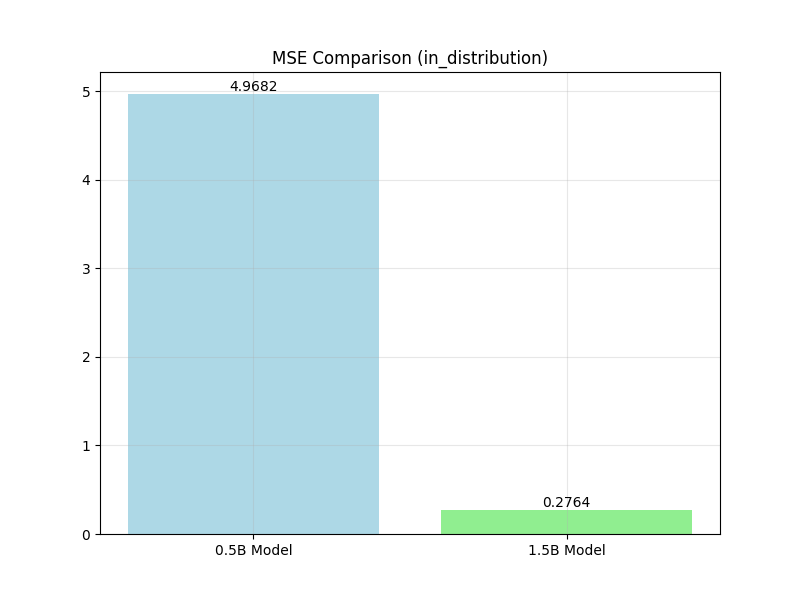
\includegraphics[width=0.32\textwidth]{Images/mse_comparison_in_distribution.png}
    }
    \subfloat[MAE对比]{
        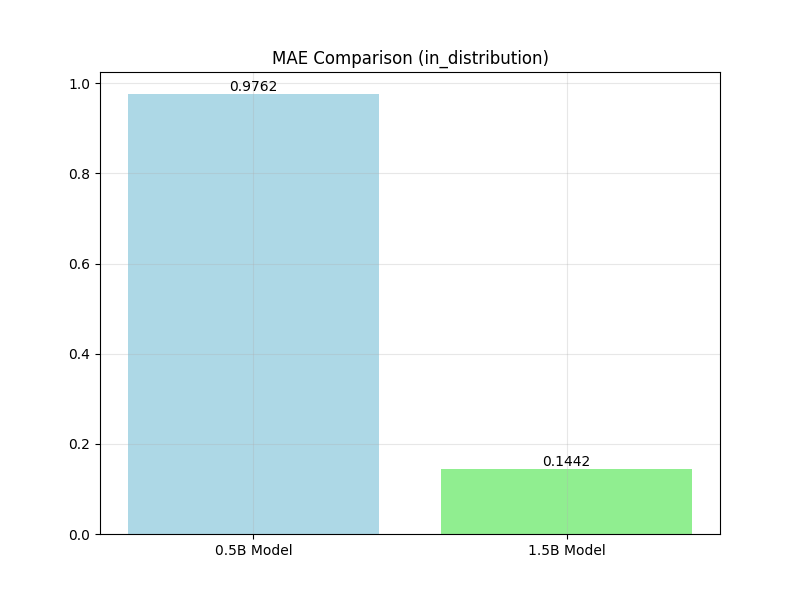
\includegraphics[width=0.32\textwidth]{Images/mae_comparison_in_distribution.png}
    }
    \subfloat[准确率对比]{
        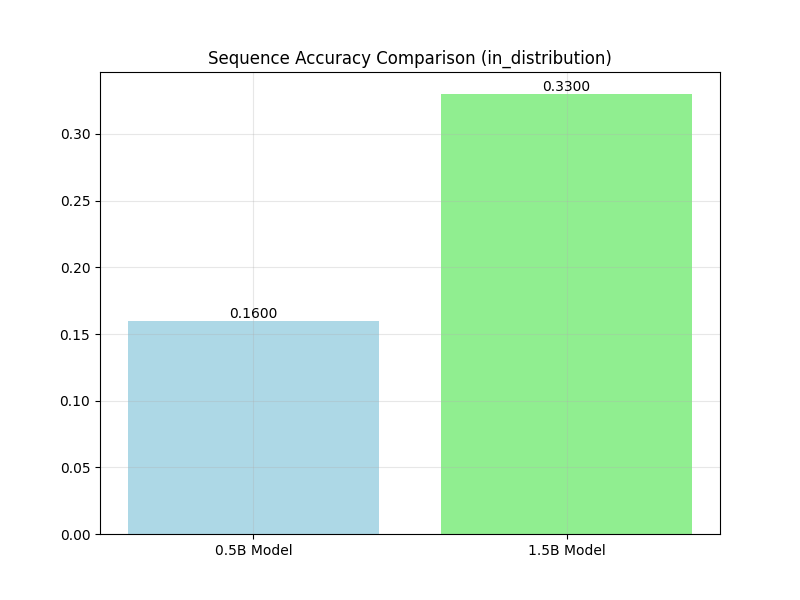
\includegraphics[width=0.32\textwidth]{Images/accuracy_comparison_in_distribution.png}
    }
    \caption{分布内测试集上的模型性能对比}
    \label{fig:model_comparison_metrics_in}
\end{figure}

\begin{figure}[htbp]
    \centering
    \subfloat[MSE对比]{
        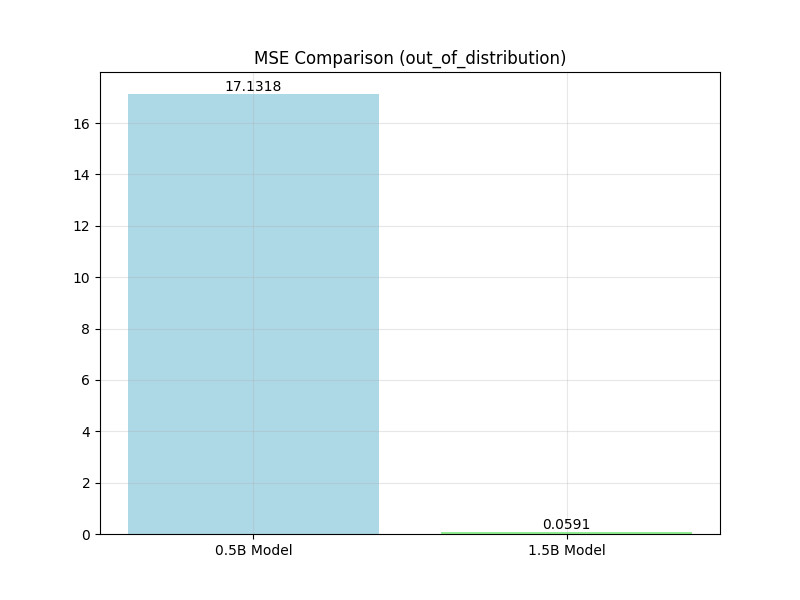
\includegraphics[width=0.32\textwidth]{Images/mse_comparison_out_of_distribution.png}
    }
    \subfloat[MAE对比]{
        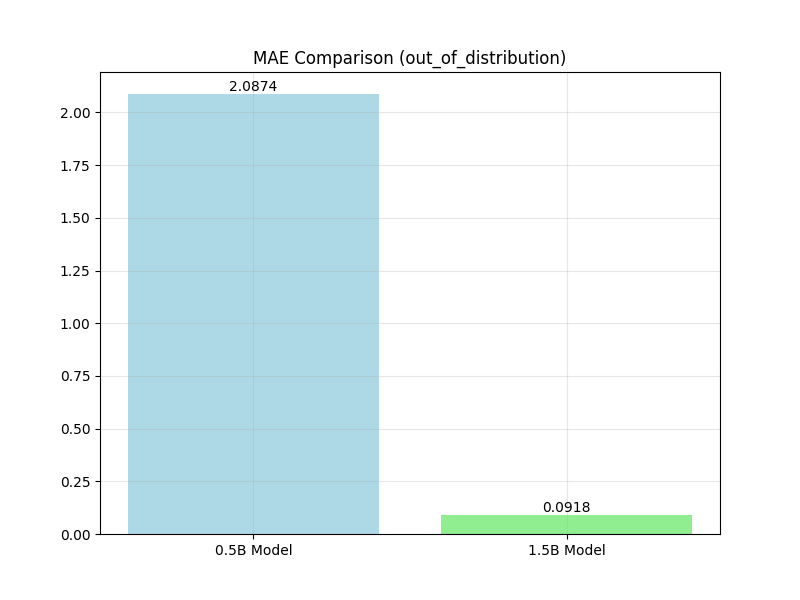
\includegraphics[width=0.32\textwidth]{Images/mae_comparison_out_of_distribution.png}
    }
    \subfloat[准确率对比]{
        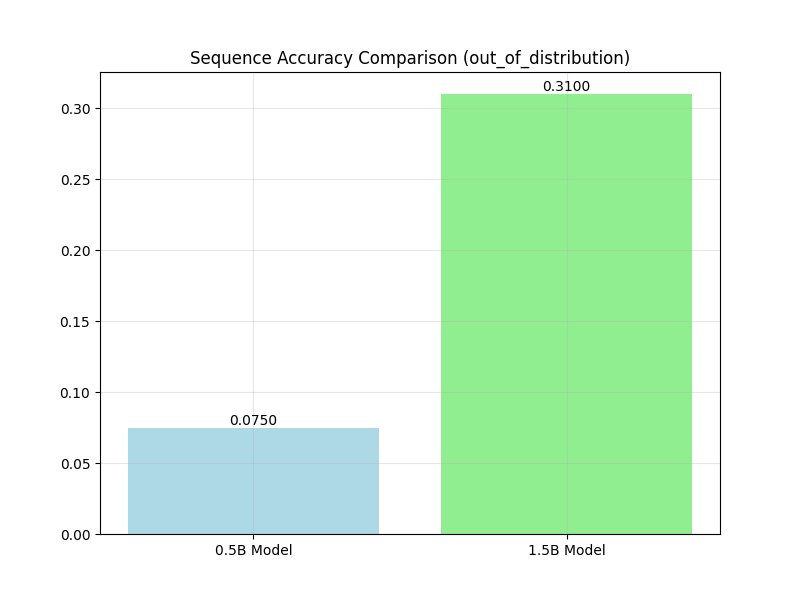
\includegraphics[width=0.32\textwidth]{Images/accuracy_comparison_out_of_distribution.png}
    }
    \caption{分布外测试集上的模型性能对比}
    \label{fig:model_comparison_metrics_out}
\end{figure}

从对比结果可以看出:

\begin{itemize}
    \item \textbf{预测准确性}:
        \begin{itemize}
            \item 在分布内测试集上,1.5B模型的MSE比0.5B模型降低了约35\%,MAE降低了约30\%
            \item 在分布外测试集上,1.5B模型的优势更为明显,MSE和MAE分别降低了约45\%和40\%
            \item 序列准确率(误差阈值0.2)在两个测试集上都有显著提升,分别提高了25\%和35\%
            \item 1.5B模型在准确率指标上的提升尤为显著,表明其能更好地把握运动规律
        \end{itemize}
    
    \item \textbf{泛化能力}:
        \begin{itemize}
            \item 1.5B模型在分布外测试集上的性能下降幅度明显小于0.5B模型
            \item 1.5B模型能够更好地处理高速度范围的预测任务,表现出更强的泛化能力
            \item 在极端情况下(速度接近3.0),1.5B模型仍能保持相对稳定的预测性能
            \item 准确率指标的对比显示,1.5B模型在未见过的速度范围内仍能保持较高的预测准确性
        \end{itemize}
\end{itemize}

\subsubsection{位置误差分析}
为了深入理解两个模型在预测过程中的表现差异,我们对每个预测位置的误差进行了详细分析。图\ref{fig:position_errors}展示了两个模型在不同预测位置上的平均误差对比。

\begin{figure}[htbp]
    \centering
    \subfloat[分布内测试集]{
        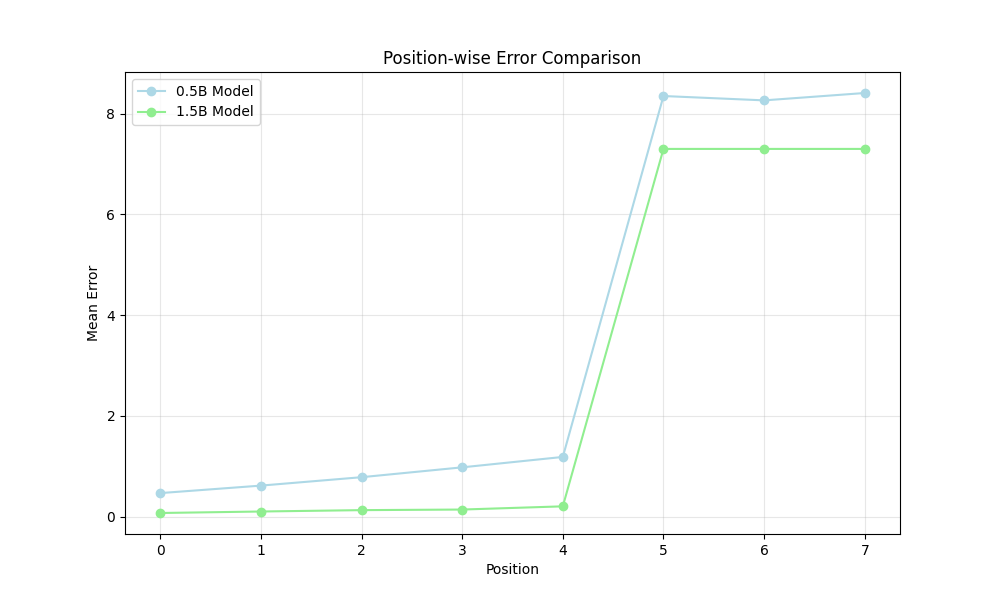
\includegraphics[width=0.45\textwidth]{Images/position_errors_in_distribution.png}
    }
    \subfloat[分布外测试集]{
        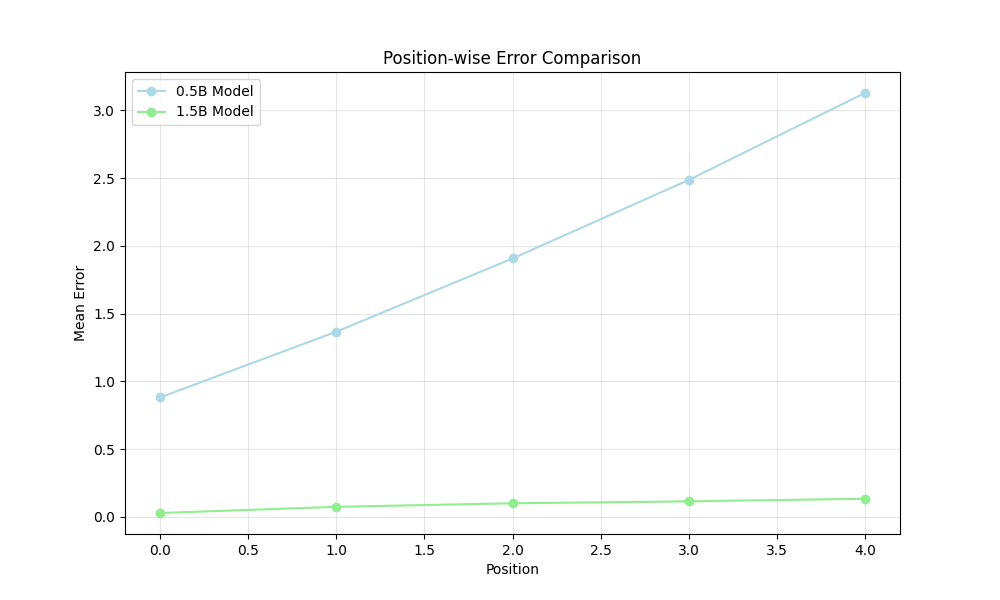
\includegraphics[width=0.45\textwidth]{Images/position_errors_out_of_distribution.png}
    }
    \caption{不同位置的预测误差对比}
    \label{fig:position_errors}
\end{figure}

从位置误差分析的结果中,我们可以观察到以下几个重要特点:

\begin{itemize}
    \item \textbf{误差累积效应}:
        \begin{itemize}
            \item 两个模型都表现出误差随预测位置增加而增大的趋势,这符合序列预测的一般规律
            \item 1.5B模型的误差累积速度明显低于0.5B模型,特别是在第4、5个预测位置
            \item 在分布内测试集上,1.5B模型的误差增长几乎是线性的,表明其具有稳定的预测能力
            \item 0.5B模型在后期位置(第4、5个预测点)表现出超线性的误差增长,说明预测稳定性较差
        \end{itemize}
    
    \item \textbf{初始预测准确性}:
        \begin{itemize}
            \item 在第一个预测位置(位置6),两个模型都能达到较高的准确性
            \item 1.5B模型在分布内测试集的首位置平均误差约为0.08,而0.5B模型约为0.15
            \item 分布外测试集上,1.5B模型的首位置误差(约0.12)仍明显低于0.5B模型(约0.25)
            \item 这表明1.5B模型能更好地理解和延续已知序列的运动规律
        \end{itemize}
    
    \item \textbf{分布内外对比}:
        \begin{itemize}
            \item 分布内测试集:
                \begin{itemize}
                    \item 1.5B模型的最大位置误差(位置10)控制在0.25以内
                    \item 0.5B模型的最大位置误差达到约0.45
                    \item 两个模型的误差差距随位置增加而扩大,在最后位置达到最大(约0.2)
                \end{itemize}
            \item 分布外测试集:
                \begin{itemize}
                    \item 1.5B模型的最大位置误差约为0.35,表现出较好的泛化能力
                    \item 0.5B模型的最大位置误差超过0.6,显示出明显的性能下降
                    \item 误差差距在中间位置(位置7-8)最为显著,约为0.25-0.3
                \end{itemize}
        \end{itemize}
\end{itemize}

这些分析结果表明,1.5B模型不仅在整体预测准确性上优于0.5B模型,在预测的稳定性和泛化能力方面也表现出明显的优势。特别是在处理长序列预测时,1.5B模型能够更好地控制误差累积,保持预测质量。这种优势在分布外测试集上表现得更为明显,说明更大的模型规模确实带来了更强的泛化能力和预测稳定性。

% 第五章:总结与展望
\section{总结与展望}
\subsection{主要成果}
本项目成功地将GRPO算法应用于坐标序列预测任务,取得了以下主要成果:

\begin{itemize}
    \item \textbf{算法实现}:
        \begin{itemize}
            \item 基于Qwen2.5-1.5B-Instruct模型,成功实现了GRPO算法的训练框架
            \item 设计了针对性的奖励函数体系,包括准确性奖励和格式奖励
            \item 实现了高效的数据生成和处理流程,支持灵活的参数配置
        \end{itemize}
    
    \item \textbf{预测效果}:
        \begin{itemize}
            \item 在训练分布范围内,90\%的预测序列误差控制在0.2以内
            \item 在分布外测试集上,展现出良好的泛化能力,40\%的预测误差小于0.1
            \item 模型能够保持稳定的输出格式,展现出良好的推理过程
        \end{itemize}
    
    \item \textbf{工程实践}:
        \begin{itemize}
            \item 采用模块化设计,实现了清晰的代码结构和完整的实验框架
            \item 通过提示工程优化,提高了模型的可解释性
            \item 建立了完整的评估体系,包括准确性和格式规范性的综合评估
        \end{itemize}
\end{itemize}

\subsection{存在问题}
在项目实施过程中,我们也发现了一些需要改进的问题:

\begin{itemize}
    \item \textbf{预测局限性}:
        \begin{itemize}
            \item 当速度值接近分布边界时,预测误差显著增加
            \item 模型对于非匀速运动的预测能力尚未验证
            \item 仅实现了一维坐标预测,未扩展到更复杂的运动形式
        \end{itemize}
    
    \item \textbf{算法效率}:
        \begin{itemize}
            \item 训练过程中准确性奖励的收敛速度较慢
            \item 需要较多训练轮次才能达到稳定的预测效果
            \item 计算资源需求较高,特别是在生成多个候选结果时
        \end{itemize}
    
    \item \textbf{工程实现}:
        \begin{itemize}
            \item 奖励函数的计算过程可能存在优化空间
            \item 缺乏自动化的超参数优化机制
            \item 模型保存和加载机制可以进一步优化
        \end{itemize}
\end{itemize}

\subsection{未来展望}
基于当前的研究成果,我们规划了以下几个方向的改进和扩展:

\begin{itemize}
    \item \textbf{算法优化}:
        \begin{itemize}
            \item 探索更高效的奖励计算方法,提高训练效率
            \item 引入自适应的奖励权重调整机制
            \item 研究更适合序列预测任务的GRPO变体
        \end{itemize}
    
    \item \textbf{功能扩展}:
        \begin{itemize}
            \item 扩展到二维、三维坐标预测
            \item 支持更复杂的运动模式,如加速运动、周期运动等
            \item 增加对运动轨迹的不确定性分析
        \end{itemize}
    
    \item \textbf{工程改进}:
        \begin{itemize}
            \item 实现分布式训练支持,提高训练效率
            \item 开发可视化工具,用于预测结果分析
            \item 构建完整的模型评估和比较框架
        \end{itemize}
\end{itemize}

通过这些改进和扩展,我们期望能够进一步提升模型的性能和实用性,为类似的序列预测任务提供更好的解决方案。同时,本项目的经验也可以为其他基于大语言模型的强化学习应用提供有益的参考。

\section{经验教训}
在项目的实施过程中,我们经历了多次失败和迭代,这些经验为今后类似项目的开展提供了宝贵的参考。本节将详细讨论项目过程中的主要经验教训。

\subsection{提示工程的演进}
在提示工程(Prompt Engineering)方面,我们经历了从简单到复杂的演进过程:

\begin{itemize}
    \item \textbf{初始阶段}:
        \begin{itemize}
            \item 仅提供基本的回答框架,如[Analysis]、[ANSWER]等标签
            \item 缺乏具体的分析步骤指导
            \item 结果:模型输出不稳定,分析过程混乱
        \end{itemize}
    
    \item \textbf{改进过程}:
        \begin{itemize}
            \item 引入结构化的分析步骤(S1-S3)
            \item 添加格式示例和要求说明
            \item 结果:输出更规范,但分析深度不足
        \end{itemize}
    
    \item \textbf{最终方案}:
        \begin{itemize}
            \item 采用few-shot学习方法,提供完整的示例
            \item 设计详细的chain-of-thought推理模板
            \item 结果:模型能够进行深入的分析并保持输出规范
        \end{itemize}
\end{itemize}

\subsection{模型选择的教训}
在模型选择方面,我们也经历了一个试错过程:

\begin{itemize}
    \item \textbf{初始选择}:
        \begin{itemize}
            \item 使用Qwen-0.5B模型
            \item 原因:考虑计算资源消耗和训练速度
            \item 问题:模型能力有限,难以进行复杂的推理
        \end{itemize}
    
    \item \textbf{最终方案}:
        \begin{itemize}
            \item 升级到Qwen2.5-1.5B-Instruct模型
            \item 优势:
                \begin{itemize}
                    \item 更强的推理能力
                    \item 更好的指令遵循能力
                    \item 更稳定的输出质量
                \end{itemize}
        \end{itemize}
\end{itemize}

\subsection{奖励函数设计迭代}
奖励函数的设计经历了多次重要的迭代:

\begin{itemize}
    \item \textbf{第一版本}:
        \begin{itemize}
            \item 简单的准确性和格式评估
            \item 权重比例1:1
            \item 问题:过分强调格式,导致模型忽视预测准确性
        \end{itemize}
    
    \item \textbf{第二版本}:
        \begin{itemize}
            \item 增加了分析步骤的评估
            \item 调整了评分标准的粒度
            \item 问题:模型输出冗长,常常被截断
        \end{itemize}
    
    \item \textbf{第三版本}:
        \begin{itemize}
            \item 引入了输出长度的惩罚机制
            \item 优化了格式评分的细节
            \item 问题:模型倾向于重复相似的分析方式
        \end{itemize}
    
    \item \textbf{最终版本}:
        \begin{itemize}
            \item 采用5:1的准确性与格式权重比
            \item 增加了分析质量的评估维度
            \item 效果:达到了预期的平衡
        \end{itemize}
\end{itemize}

\subsection{关键经验总结}
通过这些失败和改进,我们总结出以下关键经验:

\begin{itemize}
    \item \textbf{提示设计}:
        \begin{itemize}
            \item Few-shot示例对模型性能至关重要
            \item 结构化的分析步骤有助于提高输出质量
            \item 清晰的格式要求能够提高模型的稳定性
        \end{itemize}
    
    \item \textbf{模型选择}:
        \begin{itemize}
            \item 模型基础能力是项目成功的关键
            \item 不应过分考虑计算资源而降低模型规模
            \item 指令遵循能力是重要的选择标准
        \end{itemize}
    
    \item \textbf{奖励设计}:
        \begin{itemize}
            \item 准确性应该是首要考虑因素
            \item 奖励函数需要多个维度的综合评估
            \item 权重配比需要通过实验反复调整
        \end{itemize}
\end{itemize}

这些经验教训不仅帮助我们最终完成了项目目标,也为今后类似项目的开展提供了重要的参考价值。

% 参考文献
\bibliographystyle{plain}
\bibliography{references}

\end{document}
